% Chapter 13

\chapter{Numerical analysis} % Main chapter title

\label{Chapter13} % For referencing the chapter elsewhere, use \ref{Chapter12} 

\lhead{Part IV. \emph{Kitaev chain}}
\chead{Chapter 13. \emph{Numerical analysis}} % This is for the header on each page - perhaps a shortened title
%----------------------------------------------------------------------------------------
In this chapter we present the numerical analysis for the Kitaev chain in the one-dimensional Bose gas. In section \ref{sec.onlyNN} we briefly investigate the nearest neighbour only system, i.e. $t_2 = 0$. In section \ref{sec.NNNincluded} we include the next-nearest neighbour hopping and study the effect of introducing this parameter. 
 
\section{Only nearest neighbour hopping} \label{sec.onlyNN}
We numerically study the system as a function of two parameters: the coherence length, $\xi$, and the filling fraction $n = N_F/N$. We use the Bose gas parameter $n_Ba_B$ to adjust the coherence length through $\xi \propto (n_Ba_B)^{-1/2}$. We keep the interaction strength, $G$, constant. The phase diagrams are produced in the following manner. For each value of $\xi$ we compute the effective interaction using equation \eqref{eq.gapequation.lattice}. Then for each value of $n$ we come with an initial guess for the pairing. We use $\sin(kd)$, since this is the expected qualitative behaviour. Finally we use equations \eqref{eq.gapequation.lattice} and \eqref{eq.fillingfraction.lattice} to solve for the pairing and chemical potentials in a self-consistent manner for $T = 0$ only. This is done in precisely the same way as in the single and double wire system. This is iterated over $\xi > d$ and $0\leq n \leq 1$. 

The result of the analysis for $G = 4$ and $G = 8$ is shown in figure \ref{fig.phasediagram.t20}. We notice, that the plots are symmetrical around $n = 1/2$ and that a higher interaction strength leads to a narrower window of the topologically nontrivial phase of $\nu = 1$ shown in red. Finally as the coherence length grows, the topological nontrivial phase narrows. We can understand these three effects in the following manner. 

\begin{figure}
\begin{center}
% GNUPLOT: LaTeX picture with Postscript
\begingroup
  \makeatletter
  \providecommand\color[2][]{%
    \GenericError{(gnuplot) \space\space\space\@spaces}{%
      Package color not loaded in conjunction with
      terminal option `colourtext'%
    }{See the gnuplot documentation for explanation.%
    }{Either use 'blacktext' in gnuplot or load the package
      color.sty in LaTeX.}%
    \renewcommand\color[2][]{}%
  }%
  \providecommand\includegraphics[2][]{%
    \GenericError{(gnuplot) \space\space\space\@spaces}{%
      Package graphicx or graphics not loaded%
    }{See the gnuplot documentation for explanation.%
    }{The gnuplot epslatex terminal needs graphicx.sty or graphics.sty.}%
    \renewcommand\includegraphics[2][]{}%
  }%
  \providecommand\rotatebox[2]{#2}%
  \@ifundefined{ifGPcolor}{%
    \newif\ifGPcolor
    \GPcolorfalse
  }{}%
  \@ifundefined{ifGPblacktext}{%
    \newif\ifGPblacktext
    \GPblacktexttrue
  }{}%
  % define a \g@addto@macro without @ in the name:
  \let\gplgaddtomacro\g@addto@macro
  % define empty templates for all commands taking text:
  \gdef\gplbacktext{}%
  \gdef\gplfronttext{}%
  \makeatother
  \ifGPblacktext
    % no textcolor at all
    \def\colorrgb#1{}%
    \def\colorgray#1{}%
  \else
    % gray or color?
    \ifGPcolor
      \def\colorrgb#1{\color[rgb]{#1}}%
      \def\colorgray#1{\color[gray]{#1}}%
      \expandafter\def\csname LTw\endcsname{\color{white}}%
      \expandafter\def\csname LTb\endcsname{\color{black}}%
      \expandafter\def\csname LTa\endcsname{\color{black}}%
      \expandafter\def\csname LT0\endcsname{\color[rgb]{1,0,0}}%
      \expandafter\def\csname LT1\endcsname{\color[rgb]{0,1,0}}%
      \expandafter\def\csname LT2\endcsname{\color[rgb]{0,0,1}}%
      \expandafter\def\csname LT3\endcsname{\color[rgb]{1,0,1}}%
      \expandafter\def\csname LT4\endcsname{\color[rgb]{0,1,1}}%
      \expandafter\def\csname LT5\endcsname{\color[rgb]{1,1,0}}%
      \expandafter\def\csname LT6\endcsname{\color[rgb]{0,0,0}}%
      \expandafter\def\csname LT7\endcsname{\color[rgb]{1,0.3,0}}%
      \expandafter\def\csname LT8\endcsname{\color[rgb]{0.5,0.5,0.5}}%
    \else
      % gray
      \def\colorrgb#1{\color{black}}%
      \def\colorgray#1{\color[gray]{#1}}%
      \expandafter\def\csname LTw\endcsname{\color{white}}%
      \expandafter\def\csname LTb\endcsname{\color{black}}%
      \expandafter\def\csname LTa\endcsname{\color{black}}%
      \expandafter\def\csname LT0\endcsname{\color{black}}%
      \expandafter\def\csname LT1\endcsname{\color{black}}%
      \expandafter\def\csname LT2\endcsname{\color{black}}%
      \expandafter\def\csname LT3\endcsname{\color{black}}%
      \expandafter\def\csname LT4\endcsname{\color{black}}%
      \expandafter\def\csname LT5\endcsname{\color{black}}%
      \expandafter\def\csname LT6\endcsname{\color{black}}%
      \expandafter\def\csname LT7\endcsname{\color{black}}%
      \expandafter\def\csname LT8\endcsname{\color{black}}%
    \fi
  \fi
    \setlength{\unitlength}{0.0500bp}%
    \ifx\gptboxheight\undefined%
      \newlength{\gptboxheight}%
      \newlength{\gptboxwidth}%
      \newsavebox{\gptboxtext}%
    \fi%
    \setlength{\fboxrule}{0.5pt}%
    \setlength{\fboxsep}{1pt}%
\begin{picture}(7200.00,5040.00)%
    \gplgaddtomacro\gplbacktext{%
      \csname LTb\endcsname%
      \put(165,756){\makebox(0,0)[r]{\strut{}$1$}}%
      \put(165,1386){\makebox(0,0)[r]{\strut{}$2$}}%
      \put(165,2016){\makebox(0,0)[r]{\strut{}$3$}}%
      \put(165,2646){\makebox(0,0)[r]{\strut{}$4$}}%
      \put(165,3275){\makebox(0,0)[r]{\strut{}$5$}}%
      \put(165,3905){\makebox(0,0)[r]{\strut{}$6$}}%
      \put(165,4535){\makebox(0,0)[r]{\strut{}$7$}}%
      \put(360,473){\makebox(0,0){\strut{}$0$}}%
      \put(972,473){\makebox(0,0){\strut{}$0.2$}}%
      \put(1584,473){\makebox(0,0){\strut{}$0.4$}}%
      \put(2195,473){\makebox(0,0){\strut{}$0.6$}}%
      \put(2807,473){\makebox(0,0){\strut{}$0.8$}}%
      \put(3419,473){\makebox(0,0){\strut{}$1$}}%
    }%
    \gplgaddtomacro\gplfronttext{%
      \csname LTb\endcsname%
      \put(-209,2645){\rotatebox{-270}{\makebox(0,0){\strut{}$\xi / d$}}}%
      \put(1889,143){\makebox(0,0){\strut{}$n$}}%
      \put(1889,4928){\makebox(0,0){\strut{}$G = 4$}}%
    }%
    \gplgaddtomacro\gplbacktext{%
      \csname LTb\endcsname%
      \put(3584,756){\makebox(0,0)[r]{\strut{} }}%
      \put(3584,1386){\makebox(0,0)[r]{\strut{} }}%
      \put(3584,2016){\makebox(0,0)[r]{\strut{} }}%
      \put(3584,2646){\makebox(0,0)[r]{\strut{} }}%
      \put(3584,3275){\makebox(0,0)[r]{\strut{} }}%
      \put(3584,3905){\makebox(0,0)[r]{\strut{} }}%
      \put(3584,4535){\makebox(0,0)[r]{\strut{} }}%
      \put(3779,473){\makebox(0,0){\strut{}$0$}}%
      \put(4391,473){\makebox(0,0){\strut{}$0.2$}}%
      \put(5003,473){\makebox(0,0){\strut{}$0.4$}}%
      \put(5615,473){\makebox(0,0){\strut{}$0.6$}}%
      \put(6227,473){\makebox(0,0){\strut{}$0.8$}}%
      \put(6839,473){\makebox(0,0){\strut{}$1$}}%
    }%
    \gplgaddtomacro\gplfronttext{%
      \csname LTb\endcsname%
      \put(5309,143){\makebox(0,0){\strut{}$n$}}%
      \put(5309,4928){\makebox(0,0){\strut{}$G = 8$}}%
    }%
    \gplbacktext
    \put(0,0){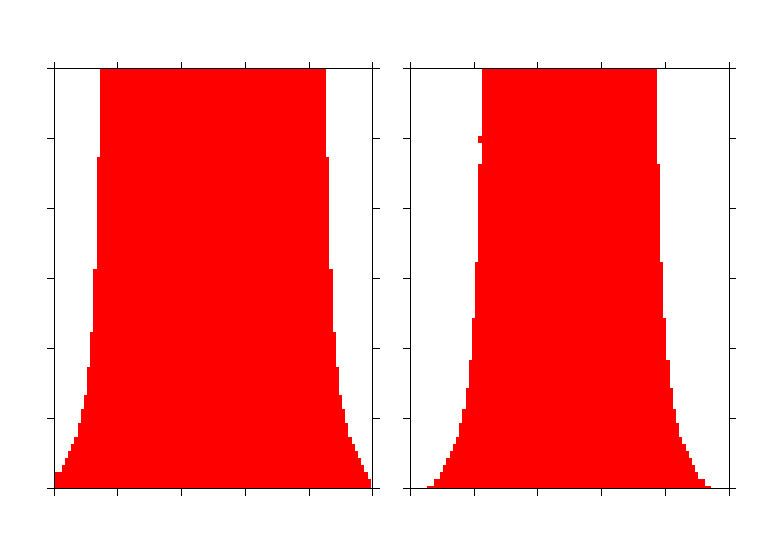
\includegraphics{Figures/Lattice.singlewire/Delta0.0/xifilldepend}}%
    \gplfronttext
  \end{picture}%
\endgroup

\caption{Phase diagrams for $G = 4$ and $G = 8$ as a function of the filling fraction $n = N_F/N$ and the coherence length $\xi$. In white: $\nu = 0$. In red: $\nu = 1$. We notice that the phase diagram for a stronger interaction exhibits a narrower window of topological nontrivial $\nu = 1$. Number of sites: $N = 100$. }
\label{fig.phasediagram.t20}
\end{center}
\end{figure}

First, the symmetry around $n = 1/2$ was discussed in section \ref{sec.fillingfractionsymmetry.breakdown}. Here we showed, that letting $n\to 1 - n$ is a symmetry of the system, if we let $\mu \to -\mu$ and $\Delta_{k} \to \Delta_{k + \pi/d}$. The topological invariant is protected under this symmetry for the following two reasons. Firstly, if $\varepsilon_k(\mu) = -t_1\cos(kd) - \mu$ crosses zero, then so does $\varepsilon_k(-\mu)$. Further, the pairing is simply shifted by $\pi / d$. This means, that there is still a contribution of $\text{sgn}(\Delta_{k_1+\pi/d})$ to the invariant from the zero of $\varepsilon_k$ in $k_1$.

Secondly, for increasing coherence lengths, $\xi$, the chemical potential must \textit{decrease}. This is because the induced interaction then attracts a larger number of neighbours lowering the total energy $E$, and thereby the chemical potential $\mu = \partial E / \partial N$. For a fixed filling fraction this eventually leads to a completely positive $\varepsilon_k = -t_1\cos(kd) - \mu$. Hereby there are no zero-points, and the invariant is zero. 

Thirdly, for a stronger interaction strength, $G$, the window of the topological phase narrows. The reason is, that when there is a nonzero interaction, the band $-t_1\cos(kd)$ can be populated eventhough $\mu$ is below the minimum of the band, i.e. $\mu < -t_1$. For a stronger interaction still, this population starts for lower and lower $\mu$ and there is a larger and larger region, where $\varepsilon_k = -t_1\cos(kd) - \mu$ is strictly positive.

The two latter effects are the same at $n$ and $1 - n$, because of the filling fraction symmetry. They can be confirmed by studying the dependency $\mu(n)$, e.g. for $G = 0, G = 4$ and $G = 8$. This results in figure \ref{fig.mun.t20.Gdepend}. We clearly observe a nonzero population in the regions with $|\mu| > t_1$ for nonzero interactions, and an increase in the size of these regions with increasing interaction strength. 

\begin{figure}
\begin{center}
% GNUPLOT: LaTeX picture with Postscript
\begingroup
  \makeatletter
  \providecommand\color[2][]{%
    \GenericError{(gnuplot) \space\space\space\@spaces}{%
      Package color not loaded in conjunction with
      terminal option `colourtext'%
    }{See the gnuplot documentation for explanation.%
    }{Either use 'blacktext' in gnuplot or load the package
      color.sty in LaTeX.}%
    \renewcommand\color[2][]{}%
  }%
  \providecommand\includegraphics[2][]{%
    \GenericError{(gnuplot) \space\space\space\@spaces}{%
      Package graphicx or graphics not loaded%
    }{See the gnuplot documentation for explanation.%
    }{The gnuplot epslatex terminal needs graphicx.sty or graphics.sty.}%
    \renewcommand\includegraphics[2][]{}%
  }%
  \providecommand\rotatebox[2]{#2}%
  \@ifundefined{ifGPcolor}{%
    \newif\ifGPcolor
    \GPcolorfalse
  }{}%
  \@ifundefined{ifGPblacktext}{%
    \newif\ifGPblacktext
    \GPblacktexttrue
  }{}%
  % define a \g@addto@macro without @ in the name:
  \let\gplgaddtomacro\g@addto@macro
  % define empty templates for all commands taking text:
  \gdef\gplbacktext{}%
  \gdef\gplfronttext{}%
  \makeatother
  \ifGPblacktext
    % no textcolor at all
    \def\colorrgb#1{}%
    \def\colorgray#1{}%
  \else
    % gray or color?
    \ifGPcolor
      \def\colorrgb#1{\color[rgb]{#1}}%
      \def\colorgray#1{\color[gray]{#1}}%
      \expandafter\def\csname LTw\endcsname{\color{white}}%
      \expandafter\def\csname LTb\endcsname{\color{black}}%
      \expandafter\def\csname LTa\endcsname{\color{black}}%
      \expandafter\def\csname LT0\endcsname{\color[rgb]{1,0,0}}%
      \expandafter\def\csname LT1\endcsname{\color[rgb]{0,1,0}}%
      \expandafter\def\csname LT2\endcsname{\color[rgb]{0,0,1}}%
      \expandafter\def\csname LT3\endcsname{\color[rgb]{1,0,1}}%
      \expandafter\def\csname LT4\endcsname{\color[rgb]{0,1,1}}%
      \expandafter\def\csname LT5\endcsname{\color[rgb]{1,1,0}}%
      \expandafter\def\csname LT6\endcsname{\color[rgb]{0,0,0}}%
      \expandafter\def\csname LT7\endcsname{\color[rgb]{1,0.3,0}}%
      \expandafter\def\csname LT8\endcsname{\color[rgb]{0.5,0.5,0.5}}%
    \else
      % gray
      \def\colorrgb#1{\color{black}}%
      \def\colorgray#1{\color[gray]{#1}}%
      \expandafter\def\csname LTw\endcsname{\color{white}}%
      \expandafter\def\csname LTb\endcsname{\color{black}}%
      \expandafter\def\csname LTa\endcsname{\color{black}}%
      \expandafter\def\csname LT0\endcsname{\color{black}}%
      \expandafter\def\csname LT1\endcsname{\color{black}}%
      \expandafter\def\csname LT2\endcsname{\color{black}}%
      \expandafter\def\csname LT3\endcsname{\color{black}}%
      \expandafter\def\csname LT4\endcsname{\color{black}}%
      \expandafter\def\csname LT5\endcsname{\color{black}}%
      \expandafter\def\csname LT6\endcsname{\color{black}}%
      \expandafter\def\csname LT7\endcsname{\color{black}}%
      \expandafter\def\csname LT8\endcsname{\color{black}}%
    \fi
  \fi
    \setlength{\unitlength}{0.0500bp}%
    \ifx\gptboxheight\undefined%
      \newlength{\gptboxheight}%
      \newlength{\gptboxwidth}%
      \newsavebox{\gptboxtext}%
    \fi%
    \setlength{\fboxrule}{0.5pt}%
    \setlength{\fboxsep}{1pt}%
\begin{picture}(7200.00,5040.00)%
    \gplgaddtomacro\gplbacktext{%
      \csname LTb\endcsname%
      \put(682,1188){\makebox(0,0)[r]{\strut{}$-2$}}%
      \csname LTb\endcsname%
      \put(682,2030){\makebox(0,0)[r]{\strut{}$-1$}}%
      \csname LTb\endcsname%
      \put(682,2872){\makebox(0,0)[r]{\strut{}$0$}}%
      \csname LTb\endcsname%
      \put(682,3713){\makebox(0,0)[r]{\strut{}$1$}}%
      \csname LTb\endcsname%
      \put(682,4555){\makebox(0,0)[r]{\strut{}$2$}}%
      \csname LTb\endcsname%
      \put(877,484){\makebox(0,0){\strut{}$0$}}%
      \csname LTb\endcsname%
      \put(2050,484){\makebox(0,0){\strut{}$0.2$}}%
      \csname LTb\endcsname%
      \put(3222,484){\makebox(0,0){\strut{}$0.4$}}%
      \csname LTb\endcsname%
      \put(4395,484){\makebox(0,0){\strut{}$0.6$}}%
      \csname LTb\endcsname%
      \put(5567,484){\makebox(0,0){\strut{}$0.8$}}%
      \csname LTb\endcsname%
      \put(6740,484){\makebox(0,0){\strut{}$1$}}%
    }%
    \gplgaddtomacro\gplfronttext{%
      \csname LTb\endcsname%
      \put(176,2871){\rotatebox{-270}{\makebox(0,0){\strut{}$\mu$}}}%
      \put(3808,154){\makebox(0,0){\strut{}$n$}}%
      \csname LTb\endcsname%
      \put(1933,4803){\makebox(0,0)[r]{\strut{}$G = 0.0$}}%
      \csname LTb\endcsname%
      \put(1933,4583){\makebox(0,0)[r]{\strut{}$G = 2.0$}}%
      \csname LTb\endcsname%
      \put(1933,4363){\makebox(0,0)[r]{\strut{}$G = 4.0$}}%
      \csname LTb\endcsname%
      \put(1933,4143){\makebox(0,0)[r]{\strut{}$G = 8.0$}}%
    }%
    \gplbacktext
    \put(0,0){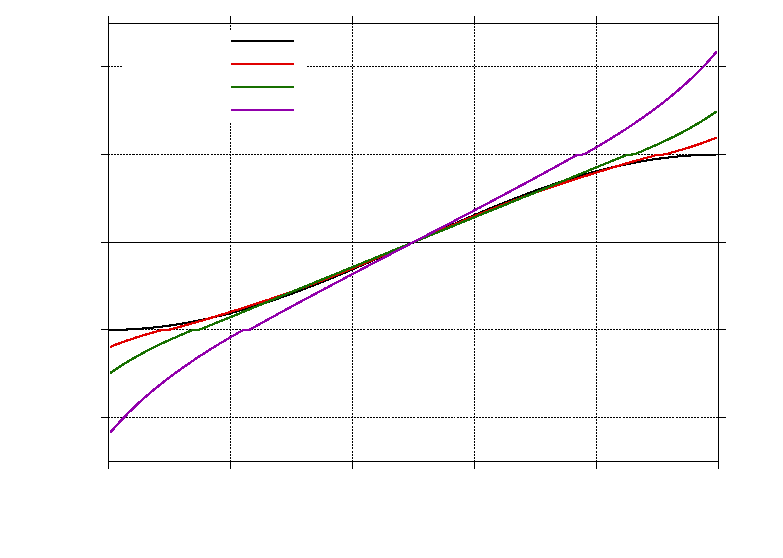
\includegraphics{Figures/Lattice.singlewire/Delta.mu.n0Gvary/ndepend}}%
    \gplfronttext
  \end{picture}%
\endgroup

\caption{The chemical potential, $\mu$, as a function of filling fraction $n$ for different interaction strengths $G$. We notice, that for nonzero interaction strengths the lattice starts populating for $|\mu| > t_1$. There is a topological phase transition exactly at $|\mu| = t_1$. $\nu = 1$ for $|\mu|< t_1$ and $\nu = 0$ for $|\mu| > t_1$. Other parameters: $N = 100, \xi / d = 8.0$}
\label{fig.mun.t20.Gdepend}
\end{center}
\end{figure}

\section{Next-nearest neighbour hopping included}
\label{sec.NNNincluded} 
In this section the program is very similar to the above. Now however, we include the next-nearest neighbour hopping, i.e. $t_2 \neq 0$. We produce two sets of phase diagrams, one for $t_2 = t_1$ and one for $t_2 = 0.63t_1$. For these two values of $t_2$ we do the following. First we search for the same solution as in the above, i.e. the start guess is $\Delta_k \propto \sin(kd)$. This produces the diagrams to the right in figures \ref{fig.phasediagram.t21.0} and \ref{fig.phasediagram.t20.63}. Next we search for a solutions with $\sin(2kd)$-like behaviour. This results in the diagrams to the left. The topological invariant is calculated according to equation \eqref{eq.topologicalinvariant}. We go into more detail with this below. The interesting part of the figures are the blue areas. These show, where it is possible to find a self-consistent solution with a topological invariant $\nu = 2$. It is exactly this sort of solution we are after!  

\begin{figure}
\begin{center}
% GNUPLOT: LaTeX picture with Postscript
\begingroup
  \makeatletter
  \providecommand\color[2][]{%
    \GenericError{(gnuplot) \space\space\space\@spaces}{%
      Package color not loaded in conjunction with
      terminal option `colourtext'%
    }{See the gnuplot documentation for explanation.%
    }{Either use 'blacktext' in gnuplot or load the package
      color.sty in LaTeX.}%
    \renewcommand\color[2][]{}%
  }%
  \providecommand\includegraphics[2][]{%
    \GenericError{(gnuplot) \space\space\space\@spaces}{%
      Package graphicx or graphics not loaded%
    }{See the gnuplot documentation for explanation.%
    }{The gnuplot epslatex terminal needs graphicx.sty or graphics.sty.}%
    \renewcommand\includegraphics[2][]{}%
  }%
  \providecommand\rotatebox[2]{#2}%
  \@ifundefined{ifGPcolor}{%
    \newif\ifGPcolor
    \GPcolorfalse
  }{}%
  \@ifundefined{ifGPblacktext}{%
    \newif\ifGPblacktext
    \GPblacktexttrue
  }{}%
  % define a \g@addto@macro without @ in the name:
  \let\gplgaddtomacro\g@addto@macro
  % define empty templates for all commands taking text:
  \gdef\gplbacktext{}%
  \gdef\gplfronttext{}%
  \makeatother
  \ifGPblacktext
    % no textcolor at all
    \def\colorrgb#1{}%
    \def\colorgray#1{}%
  \else
    % gray or color?
    \ifGPcolor
      \def\colorrgb#1{\color[rgb]{#1}}%
      \def\colorgray#1{\color[gray]{#1}}%
      \expandafter\def\csname LTw\endcsname{\color{white}}%
      \expandafter\def\csname LTb\endcsname{\color{black}}%
      \expandafter\def\csname LTa\endcsname{\color{black}}%
      \expandafter\def\csname LT0\endcsname{\color[rgb]{1,0,0}}%
      \expandafter\def\csname LT1\endcsname{\color[rgb]{0,1,0}}%
      \expandafter\def\csname LT2\endcsname{\color[rgb]{0,0,1}}%
      \expandafter\def\csname LT3\endcsname{\color[rgb]{1,0,1}}%
      \expandafter\def\csname LT4\endcsname{\color[rgb]{0,1,1}}%
      \expandafter\def\csname LT5\endcsname{\color[rgb]{1,1,0}}%
      \expandafter\def\csname LT6\endcsname{\color[rgb]{0,0,0}}%
      \expandafter\def\csname LT7\endcsname{\color[rgb]{1,0.3,0}}%
      \expandafter\def\csname LT8\endcsname{\color[rgb]{0.5,0.5,0.5}}%
    \else
      % gray
      \def\colorrgb#1{\color{black}}%
      \def\colorgray#1{\color[gray]{#1}}%
      \expandafter\def\csname LTw\endcsname{\color{white}}%
      \expandafter\def\csname LTb\endcsname{\color{black}}%
      \expandafter\def\csname LTa\endcsname{\color{black}}%
      \expandafter\def\csname LT0\endcsname{\color{black}}%
      \expandafter\def\csname LT1\endcsname{\color{black}}%
      \expandafter\def\csname LT2\endcsname{\color{black}}%
      \expandafter\def\csname LT3\endcsname{\color{black}}%
      \expandafter\def\csname LT4\endcsname{\color{black}}%
      \expandafter\def\csname LT5\endcsname{\color{black}}%
      \expandafter\def\csname LT6\endcsname{\color{black}}%
      \expandafter\def\csname LT7\endcsname{\color{black}}%
      \expandafter\def\csname LT8\endcsname{\color{black}}%
    \fi
  \fi
    \setlength{\unitlength}{0.0500bp}%
    \ifx\gptboxheight\undefined%
      \newlength{\gptboxheight}%
      \newlength{\gptboxwidth}%
      \newsavebox{\gptboxtext}%
    \fi%
    \setlength{\fboxrule}{0.5pt}%
    \setlength{\fboxsep}{1pt}%
\begin{picture}(7200.00,5040.00)%
    \gplgaddtomacro\gplbacktext{%
      \csname LTb\endcsname%
      \put(165,756){\makebox(0,0)[r]{\strut{}$1$}}%
      \put(165,1386){\makebox(0,0)[r]{\strut{}$2$}}%
      \put(165,2016){\makebox(0,0)[r]{\strut{}$3$}}%
      \put(165,2646){\makebox(0,0)[r]{\strut{}$4$}}%
      \put(165,3275){\makebox(0,0)[r]{\strut{}$5$}}%
      \put(165,3905){\makebox(0,0)[r]{\strut{}$6$}}%
      \put(165,4535){\makebox(0,0)[r]{\strut{}$7$}}%
      \put(360,473){\makebox(0,0){\strut{}$0$}}%
      \put(972,473){\makebox(0,0){\strut{}$0.2$}}%
      \put(1584,473){\makebox(0,0){\strut{}$0.4$}}%
      \put(2195,473){\makebox(0,0){\strut{}$0.6$}}%
      \put(2807,473){\makebox(0,0){\strut{}$0.8$}}%
      \put(3419,473){\makebox(0,0){\strut{}$1$}}%
    }%
    \gplgaddtomacro\gplfronttext{%
      \csname LTb\endcsname%
      \put(-209,2645){\rotatebox{-270}{\makebox(0,0){\strut{}$\xi / d$}}}%
      \put(1889,143){\makebox(0,0){\strut{}$n$}}%
      \put(1889,4928){\makebox(0,0){\strut{}$t_2 = t_1, \text{anomalous}$}}%
      \put(972,3590){\makebox(0,0){\color{white}\strut{}$\nu = 1$}}%
      \put(1889, 3590){\makebox(0,0){\color{white}\strut{}$\nu = 2$}}%
      \put(2807,3590){\makebox(0,0){\strut{}$\nu = 0$}}%
      \put(972,3275){\makebox(0,0){\color{white}\strut{}$\times$}}%
      \put(1890,3275){\makebox(0,0){\color{white}\strut{}$*$}}%
    }%
    \gplgaddtomacro\gplbacktext{%
      \csname LTb\endcsname%
      \put(3584,756){\makebox(0,0)[r]{\strut{} }}%
      \put(3584,1386){\makebox(0,0)[r]{\strut{} }}%
      \put(3584,2016){\makebox(0,0)[r]{\strut{} }}%
      \put(3584,2646){\makebox(0,0)[r]{\strut{} }}%
      \put(3584,3275){\makebox(0,0)[r]{\strut{} }}%
      \put(3584,3905){\makebox(0,0)[r]{\strut{} }}%
      \put(3584,4535){\makebox(0,0)[r]{\strut{} }}%
      \put(3779,473){\makebox(0,0){\strut{}$0$}}%
      \put(4391,473){\makebox(0,0){\strut{}$0.2$}}%
      \put(5003,473){\makebox(0,0){\strut{}$0.4$}}%
      \put(5615,473){\makebox(0,0){\strut{}$0.6$}}%
      \put(6227,473){\makebox(0,0){\strut{}$0.8$}}%
      \put(6839,473){\makebox(0,0){\strut{}$1$}}%
    }%
    \gplgaddtomacro\gplfronttext{%
      \csname LTb\endcsname%
      \put(5309,143){\makebox(0,0){\strut{}$n$}}%
      \put(5309,4928){\makebox(0,0){\strut{}$t_2 = t_1, \text{normal}$}}%
      \put(4391,3590){\makebox(0,0){\color{white}\strut{}$\nu = 1$}}%
      \put(6227,3590){\makebox(0,0){\strut{}$\nu = 0$}}%
      \put(4391,3275){\makebox(0,0){\color{white}\strut{}$\times$}}%
      \put(5309,3275){\makebox(0,0){\strut{}$*$}}%
    }%
    \gplbacktext
    \put(0,0){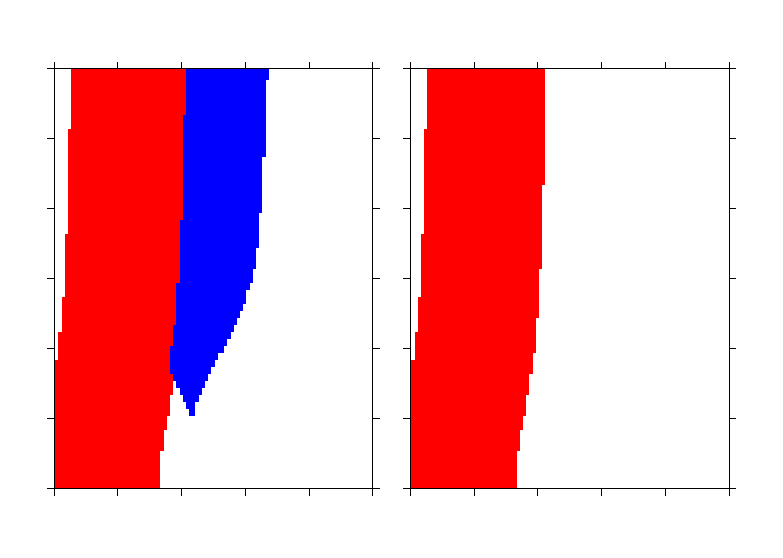
\includegraphics{Figures/Lattice.singlewire/t2nonzerophasediagrams/xifilldepend1}}%
    \gplfronttext
  \end{picture}%
\endgroup

\caption{Topological phase diagram for $t_2 = t_1$ as a function of the filling fraction $n = N_F/N$ and the coherence length $\xi$. Invariant: in white: $\nu = 0$, in red: $\nu = 1$, in blue: $\nu = 2$. To the left: (anomalous) result of searching for $\Delta_k\propto \sin(2kd)$-like solutions. To the right: (normal) result of searching for $\Delta_k \propto \sin(kd)$-like solutions. The algorithm is a little uncertain around the blue tip at $n \approx 0.4, \xi / d \approx 2$. The phase has here been checked by doubling the number of lattice sites. Other parameters: $G = 4$, $N = 100$. }
\label{fig.phasediagram.t21.0}
\vspace{0.5cm}
% GNUPLOT: LaTeX picture with Postscript
\begingroup
  \makeatletter
  \providecommand\color[2][]{%
    \GenericError{(gnuplot) \space\space\space\@spaces}{%
      Package color not loaded in conjunction with
      terminal option `colourtext'%
    }{See the gnuplot documentation for explanation.%
    }{Either use 'blacktext' in gnuplot or load the package
      color.sty in LaTeX.}%
    \renewcommand\color[2][]{}%
  }%
  \providecommand\includegraphics[2][]{%
    \GenericError{(gnuplot) \space\space\space\@spaces}{%
      Package graphicx or graphics not loaded%
    }{See the gnuplot documentation for explanation.%
    }{The gnuplot epslatex terminal needs graphicx.sty or graphics.sty.}%
    \renewcommand\includegraphics[2][]{}%
  }%
  \providecommand\rotatebox[2]{#2}%
  \@ifundefined{ifGPcolor}{%
    \newif\ifGPcolor
    \GPcolorfalse
  }{}%
  \@ifundefined{ifGPblacktext}{%
    \newif\ifGPblacktext
    \GPblacktexttrue
  }{}%
  % define a \g@addto@macro without @ in the name:
  \let\gplgaddtomacro\g@addto@macro
  % define empty templates for all commands taking text:
  \gdef\gplbacktext{}%
  \gdef\gplfronttext{}%
  \makeatother
  \ifGPblacktext
    % no textcolor at all
    \def\colorrgb#1{}%
    \def\colorgray#1{}%
  \else
    % gray or color?
    \ifGPcolor
      \def\colorrgb#1{\color[rgb]{#1}}%
      \def\colorgray#1{\color[gray]{#1}}%
      \expandafter\def\csname LTw\endcsname{\color{white}}%
      \expandafter\def\csname LTb\endcsname{\color{black}}%
      \expandafter\def\csname LTa\endcsname{\color{black}}%
      \expandafter\def\csname LT0\endcsname{\color[rgb]{1,0,0}}%
      \expandafter\def\csname LT1\endcsname{\color[rgb]{0,1,0}}%
      \expandafter\def\csname LT2\endcsname{\color[rgb]{0,0,1}}%
      \expandafter\def\csname LT3\endcsname{\color[rgb]{1,0,1}}%
      \expandafter\def\csname LT4\endcsname{\color[rgb]{0,1,1}}%
      \expandafter\def\csname LT5\endcsname{\color[rgb]{1,1,0}}%
      \expandafter\def\csname LT6\endcsname{\color[rgb]{0,0,0}}%
      \expandafter\def\csname LT7\endcsname{\color[rgb]{1,0.3,0}}%
      \expandafter\def\csname LT8\endcsname{\color[rgb]{0.5,0.5,0.5}}%
    \else
      % gray
      \def\colorrgb#1{\color{black}}%
      \def\colorgray#1{\color[gray]{#1}}%
      \expandafter\def\csname LTw\endcsname{\color{white}}%
      \expandafter\def\csname LTb\endcsname{\color{black}}%
      \expandafter\def\csname LTa\endcsname{\color{black}}%
      \expandafter\def\csname LT0\endcsname{\color{black}}%
      \expandafter\def\csname LT1\endcsname{\color{black}}%
      \expandafter\def\csname LT2\endcsname{\color{black}}%
      \expandafter\def\csname LT3\endcsname{\color{black}}%
      \expandafter\def\csname LT4\endcsname{\color{black}}%
      \expandafter\def\csname LT5\endcsname{\color{black}}%
      \expandafter\def\csname LT6\endcsname{\color{black}}%
      \expandafter\def\csname LT7\endcsname{\color{black}}%
      \expandafter\def\csname LT8\endcsname{\color{black}}%
    \fi
  \fi
    \setlength{\unitlength}{0.0500bp}%
    \ifx\gptboxheight\undefined%
      \newlength{\gptboxheight}%
      \newlength{\gptboxwidth}%
      \newsavebox{\gptboxtext}%
    \fi%
    \setlength{\fboxrule}{0.5pt}%
    \setlength{\fboxsep}{1pt}%
\begin{picture}(7200.00,5040.00)%
    \gplgaddtomacro\gplbacktext{%
      \csname LTb\endcsname%
      \put(165,756){\makebox(0,0)[r]{\strut{}$1$}}%
      \put(165,1386){\makebox(0,0)[r]{\strut{}$2$}}%
      \put(165,2016){\makebox(0,0)[r]{\strut{}$3$}}%
      \put(165,2646){\makebox(0,0)[r]{\strut{}$4$}}%
      \put(165,3275){\makebox(0,0)[r]{\strut{}$5$}}%
      \put(165,3905){\makebox(0,0)[r]{\strut{}$6$}}%
      \put(165,4535){\makebox(0,0)[r]{\strut{}$7$}}%
      \put(360,473){\makebox(0,0){\strut{}$0$}}%
      \put(972,473){\makebox(0,0){\strut{}$0.2$}}%
      \put(1584,473){\makebox(0,0){\strut{}$0.4$}}%
      \put(2195,473){\makebox(0,0){\strut{}$0.6$}}%
      \put(2807,473){\makebox(0,0){\strut{}$0.8$}}%
      \put(3419,473){\makebox(0,0){\strut{}$1$}}%
    }%
    \gplgaddtomacro\gplfronttext{%
      \csname LTb\endcsname%
      \put(-209,2645){\rotatebox{-270}{\makebox(0,0){\strut{}$\xi / d$}}}%
      \put(1889,143){\makebox(0,0){\strut{}$n$}}%
      \put(1889,4928){\makebox(0,0){\strut{}$t_2 = 0.63t_1, \text{anomalous}$}}%
    }%
    \gplgaddtomacro\gplbacktext{%
      \csname LTb\endcsname%
      \put(3584,756){\makebox(0,0)[r]{\strut{} }}%
      \put(3584,1386){\makebox(0,0)[r]{\strut{} }}%
      \put(3584,2016){\makebox(0,0)[r]{\strut{} }}%
      \put(3584,2646){\makebox(0,0)[r]{\strut{} }}%
      \put(3584,3275){\makebox(0,0)[r]{\strut{} }}%
      \put(3584,3905){\makebox(0,0)[r]{\strut{} }}%
      \put(3584,4535){\makebox(0,0)[r]{\strut{} }}%
      \put(3779,473){\makebox(0,0){\strut{}$0$}}%
      \put(4391,473){\makebox(0,0){\strut{}$0.2$}}%
      \put(5003,473){\makebox(0,0){\strut{}$0.4$}}%
      \put(5615,473){\makebox(0,0){\strut{}$0.6$}}%
      \put(6227,473){\makebox(0,0){\strut{}$0.8$}}%
      \put(6839,473){\makebox(0,0){\strut{}$1$}}%
    }%
    \gplgaddtomacro\gplfronttext{%
      \csname LTb\endcsname%
      \put(5309,143){\makebox(0,0){\strut{}$n$}}%
      \put(5309,4928){\makebox(0,0){\strut{}$t_2 = 0.63t_1, \text{normal}$}}%
    }%
    \gplbacktext
    \put(0,0){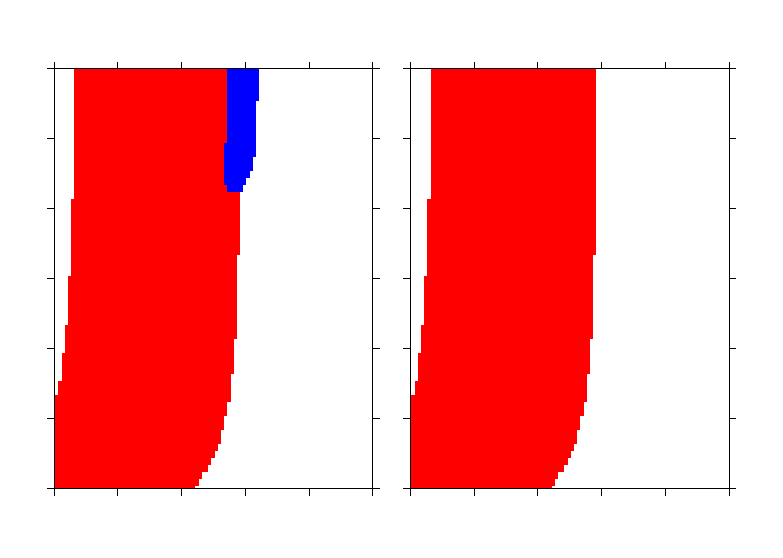
\includegraphics{Figures/Lattice.singlewire/t2nonzerophasediagrams/xifilldepend2}}%
    \gplfronttext
  \end{picture}%
\endgroup

\caption{Topological phase diagrams for $t_2 = 0.63t_1$ as a function of the filling fraction $n = N_F/N$ and the coherence length $\xi$. In white: $\nu = 0$, in red: $\nu = 1$, in blue: $\nu = 2$. To the left: (anomalous) result of searching for $\Delta_k\propto \sin(2kd)$-like solutions. To the right: (normal) result of searching for $\Delta_k \propto \sin(kd)$-like solutions. Other parameters: $G = 4$, $N = 100$. }
\label{fig.phasediagram.t20.63}
\end{center}
\end{figure}

In figure \ref{fig.Deltaexamples.t21.0} we go into more detail with the pairing at the points $(i)$ and $(ii)$ specified in figure \ref{fig.phasediagram.t21.0}. Remember, that the topological invariant depends on both the kinetic energy, $\varepsilon_k$, and the pairing, $\Delta_k$. Every zero of $\varepsilon_k$ for $k > 0$ contributes the sign of the pairing times the sign of the slope of $\varepsilon_k$. 

 At $(i)$ we only find one solution for the pairing, irrespective of the initial guess. This single solution is $\sin(kd)$-like in that it only crosses zero at $k = 0$. 




However, this is not the case in the entire red region of topological invariant $\nu = 1$. Closer to the point $(ii)$, but still in the red region, we indeed find $\sin(2kd)$-like solutions. These however still have $\nu = 1$, because the filling fraction is too low to make an additional pair of zeroes of $\varepsilon_k$. At $(ii)$ we find two solutions for the pairing. Here both a (normal) $\sin(kd)$- and an (anomalous) $\sin(2kd)$-like solution are self-consistent. Since $\varepsilon_k$ now has two pairs of zeroes, the topological invariant is $\nu = 0$ and $\nu = 2$ for the normal and anomalous pairing respectively.   


\begin{figure}
\begin{center}
% GNUPLOT: LaTeX picture with Postscript
\begingroup
  \makeatletter
  \providecommand\color[2][]{%
    \GenericError{(gnuplot) \space\space\space\@spaces}{%
      Package color not loaded in conjunction with
      terminal option `colourtext'%
    }{See the gnuplot documentation for explanation.%
    }{Either use 'blacktext' in gnuplot or load the package
      color.sty in LaTeX.}%
    \renewcommand\color[2][]{}%
  }%
  \providecommand\includegraphics[2][]{%
    \GenericError{(gnuplot) \space\space\space\@spaces}{%
      Package graphicx or graphics not loaded%
    }{See the gnuplot documentation for explanation.%
    }{The gnuplot epslatex terminal needs graphicx.sty or graphics.sty.}%
    \renewcommand\includegraphics[2][]{}%
  }%
  \providecommand\rotatebox[2]{#2}%
  \@ifundefined{ifGPcolor}{%
    \newif\ifGPcolor
    \GPcolorfalse
  }{}%
  \@ifundefined{ifGPblacktext}{%
    \newif\ifGPblacktext
    \GPblacktexttrue
  }{}%
  % define a \g@addto@macro without @ in the name:
  \let\gplgaddtomacro\g@addto@macro
  % define empty templates for all commands taking text:
  \gdef\gplbacktext{}%
  \gdef\gplfronttext{}%
  \makeatother
  \ifGPblacktext
    % no textcolor at all
    \def\colorrgb#1{}%
    \def\colorgray#1{}%
  \else
    % gray or color?
    \ifGPcolor
      \def\colorrgb#1{\color[rgb]{#1}}%
      \def\colorgray#1{\color[gray]{#1}}%
      \expandafter\def\csname LTw\endcsname{\color{white}}%
      \expandafter\def\csname LTb\endcsname{\color{black}}%
      \expandafter\def\csname LTa\endcsname{\color{black}}%
      \expandafter\def\csname LT0\endcsname{\color[rgb]{1,0,0}}%
      \expandafter\def\csname LT1\endcsname{\color[rgb]{0,1,0}}%
      \expandafter\def\csname LT2\endcsname{\color[rgb]{0,0,1}}%
      \expandafter\def\csname LT3\endcsname{\color[rgb]{1,0,1}}%
      \expandafter\def\csname LT4\endcsname{\color[rgb]{0,1,1}}%
      \expandafter\def\csname LT5\endcsname{\color[rgb]{1,1,0}}%
      \expandafter\def\csname LT6\endcsname{\color[rgb]{0,0,0}}%
      \expandafter\def\csname LT7\endcsname{\color[rgb]{1,0.3,0}}%
      \expandafter\def\csname LT8\endcsname{\color[rgb]{0.5,0.5,0.5}}%
    \else
      % gray
      \def\colorrgb#1{\color{black}}%
      \def\colorgray#1{\color[gray]{#1}}%
      \expandafter\def\csname LTw\endcsname{\color{white}}%
      \expandafter\def\csname LTb\endcsname{\color{black}}%
      \expandafter\def\csname LTa\endcsname{\color{black}}%
      \expandafter\def\csname LT0\endcsname{\color{black}}%
      \expandafter\def\csname LT1\endcsname{\color{black}}%
      \expandafter\def\csname LT2\endcsname{\color{black}}%
      \expandafter\def\csname LT3\endcsname{\color{black}}%
      \expandafter\def\csname LT4\endcsname{\color{black}}%
      \expandafter\def\csname LT5\endcsname{\color{black}}%
      \expandafter\def\csname LT6\endcsname{\color{black}}%
      \expandafter\def\csname LT7\endcsname{\color{black}}%
      \expandafter\def\csname LT8\endcsname{\color{black}}%
    \fi
  \fi
    \setlength{\unitlength}{0.0500bp}%
    \ifx\gptboxheight\undefined%
      \newlength{\gptboxheight}%
      \newlength{\gptboxwidth}%
      \newsavebox{\gptboxtext}%
    \fi%
    \setlength{\fboxrule}{0.5pt}%
    \setlength{\fboxsep}{1pt}%
\begin{picture}(7200.00,5040.00)%
    \gplgaddtomacro\gplbacktext{%
      \csname LTb\endcsname%
      \put(165,869){\makebox(0,0)[r]{\strut{}$-2$}}%
      \csname LTb\endcsname%
      \put(165,1600){\makebox(0,0)[r]{\strut{}$-1$}}%
      \csname LTb\endcsname%
      \put(165,2331){\makebox(0,0)[r]{\strut{}$0$}}%
      \csname LTb\endcsname%
      \put(165,3061){\makebox(0,0)[r]{\strut{}$1$}}%
      \csname LTb\endcsname%
      \put(165,3792){\makebox(0,0)[r]{\strut{}$2$}}%
      \csname LTb\endcsname%
      \put(429,221){\makebox(0,0){\strut{}$-3$}}%
      \csname LTb\endcsname%
      \put(916,221){\makebox(0,0){\strut{}$-2$}}%
      \csname LTb\endcsname%
      \put(1403,221){\makebox(0,0){\strut{}$-1$}}%
      \csname LTb\endcsname%
      \put(1890,221){\makebox(0,0){\strut{}$0$}}%
      \csname LTb\endcsname%
      \put(2376,221){\makebox(0,0){\strut{}$1$}}%
      \csname LTb\endcsname%
      \put(2863,221){\makebox(0,0){\strut{}$2$}}%
      \csname LTb\endcsname%
      \put(3350,221){\makebox(0,0){\strut{}$3$}}%
    }%
    \gplgaddtomacro\gplfronttext{%
      \csname LTb\endcsname%
      \put(-341,2330){\rotatebox{-270}{\makebox(0,0){\strut{}$2\Delta_k, \varepsilon_k$}}}%
      \put(1889,-109){\makebox(0,0){\strut{}$kd$}}%
      \put(429,4550){\makebox(0,0){\strut{}$(i)$}}%
      \csname LTb\endcsname%
      \put(670,4867){\makebox(0,0)[l]{\strut{}$\Delta_k/t_1 \sim \sin(1kd)$}}%
      \csname LTb\endcsname%
      \put(670,4647){\makebox(0,0)[l]{\strut{}$\varepsilon_k / t_1$}}%
    }%
    \gplgaddtomacro\gplbacktext{%
      \csname LTb\endcsname%
      \put(3584,869){\makebox(0,0)[r]{\strut{} }}%
      \csname LTb\endcsname%
      \put(3584,1600){\makebox(0,0)[r]{\strut{} }}%
      \csname LTb\endcsname%
      \put(3584,2331){\makebox(0,0)[r]{\strut{} }}%
      \csname LTb\endcsname%
      \put(3584,3061){\makebox(0,0)[r]{\strut{} }}%
      \csname LTb\endcsname%
      \put(3584,3792){\makebox(0,0)[r]{\strut{} }}%
      \csname LTb\endcsname%
      \put(3848,221){\makebox(0,0){\strut{}$-3$}}%
      \csname LTb\endcsname%
      \put(4335,221){\makebox(0,0){\strut{}$-2$}}%
      \csname LTb\endcsname%
      \put(4822,221){\makebox(0,0){\strut{}$-1$}}%
      \csname LTb\endcsname%
      \put(5309,221){\makebox(0,0){\strut{}$0$}}%
      \csname LTb\endcsname%
      \put(5796,221){\makebox(0,0){\strut{}$1$}}%
      \csname LTb\endcsname%
      \put(6283,221){\makebox(0,0){\strut{}$2$}}%
      \csname LTb\endcsname%
      \put(6770,221){\makebox(0,0){\strut{}$3$}}%
    }%
    \gplgaddtomacro\gplfronttext{%
      \csname LTb\endcsname%
      \put(5309,-109){\makebox(0,0){\strut{}$kd$}}%
      \put(3848,4550){\makebox(0,0){\strut{}$(ii)$}}%
      \csname LTb\endcsname%
      \put(4089,4867){\makebox(0,0)[l]{\strut{}$\Delta_k/t_1 \sim \sin(1kd)$}}%
      \csname LTb\endcsname%
      \put(4089,4647){\makebox(0,0)[l]{\strut{}$\Delta_k/t_1 \sim \sin(2kd)$}}%
      \csname LTb\endcsname%
      \put(4089,4427){\makebox(0,0)[l]{\strut{}$\varepsilon_k / t_1$}}%
    }%
    \gplbacktext
    \put(0,0){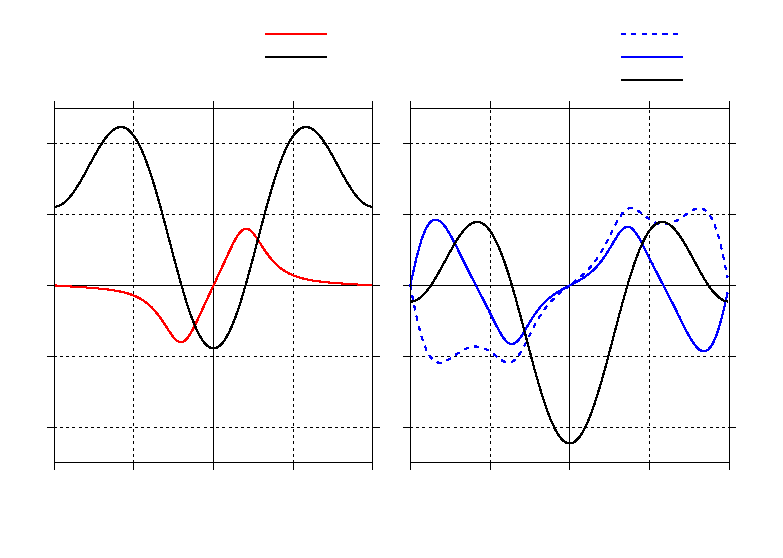
\includegraphics{Figures/Lattice.singlewire/Deltaexamples/kdepend}}%
    \gplfronttext
  \end{picture}%
\endgroup

\caption{The pairing, $\Delta_k$, and kinetic energy, $\varepsilon_k$, across the Brillouin zone. In black: $\varepsilon_k$. $(i)$, red solid line: only one solution for $\Delta_k$. This is $\sin(kd)$-like. Topological invariant: $\nu = 1$. $(ii)$, blue lines: two solutions for $\Delta_k$. Dashed blue line: $\sin(kd)$-like solution with $\nu = 0$. Solid blue line: $\sin(2kd)$-like solution with $\nu = 2$. Notice that the pairing is maximal around the zeroes of $\varepsilon_k$. Parameters: $G = 4$, $N = 100$, $\xi / d = 5$. $(i)$: $n = 0.2$, $(ii)$: $n = 0.5$.}
\label{fig.Deltaexamples.t21.0}
\end{center}
\end{figure}

